\section{Equivalent Circuits}
\begin{minipage}[l]{0.7\linewidth}
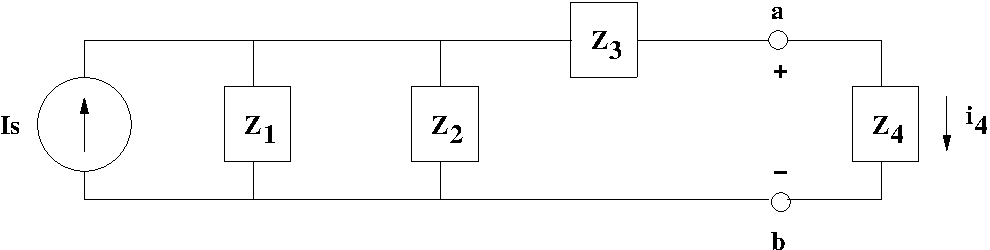
\includegraphics[width=0.9\linewidth]{thevenin/thevenin}
\end{minipage}\hfill
\begin{minipage}[l]{0.3\linewidth}
$I_s(t) = 10 \cos(1000t)$ mA\\
$Z_1$ = 20 $\Omega$\\
$Z_2$ = 30 $\Omega$\\ 
$Z_3$ = ?\\ 
$Z_4$ = variable load\\
\end{minipage}

$Z_{1..4}$ represent discrete components in the circuit (i.e., resistors,
capacitors, and inductors).  When $Z_4 = \infty$ (open circuit across terminals
$a$ \& $b$), $v_{ab} = 120\cos(1000t)$ mV, and when $Z_4 = 0$ (short circuit
across terminals $a$ to $b$), $i_4 = 9.86\cos(1000t + 9.46^\circ)$ mA.

\begin{enumerate}
    \item What is the Norton impedance ($Z_N$) for the circuit as seen from
        $Z_4$ (i.e., $Z_4$ acts as the load)?

    \item Given $Z_N$, what is $Z_3$?

    \item Is $Z_3$ a resistor, a capacitor, or an inductor?  What is the value
        of this component? 

    \item Solve for $i_4(t)$ if $Z_4$ is a 5 mH inductor. 

    \item Solve for $v_{ab}(t)$ if $Z_4$ is a 5 mH inductor (same as (d)). 
\end{enumerate}
